% lint-skip: 未完成ステータス（figure/table caption 未対応，人手チェック時に解消予定）
\documentclass[../../main.tex]{subfiles}
\begin{document}

\begin{flushright}
  \footnotesize\textit{【自動文字起こし・要確認】}
\end{flushright}

[解] $C: x^2 + \left(y - \dfrac{2-p}{2}\right)^2 = \left(\dfrac{2+p}{2}\right)^2$

だから，これと $y=1$ の交点の $x$ 座標は

$x = \pm \sqrt{p+1}$ である．従って，$Q(s, t)$

に対し $s > 0$ から
\[
  \begin{cases}
    \dfrac{s}{2} = \sqrt{p+1} \\
    \dfrac{t-p}{2} = 1
  \end{cases}
\]
$\Leftrightarrow s = 2\sqrt{p+1}, \ t = 2+p \cdots (1)$

である．よって
\[ s^2 = 4(p+1) \quad \therefore \ p = \dfrac{s^2}{4} - 1 \quad (p > 0 \text{ から } s > 2) \]
だから代入して
\[ t = 2 + \dfrac{s^2}{4} - 1 = \dfrac{1}{4}s^2 + 1 \]
より，求めるキセキは
\[ y = \dfrac{1}{4}x^2 + 1 \quad (x > 2) \]
であり，$x = 2\sqrt{p+1}$ での接線は
\[ l: y = \sqrt{p+1}x - p \]
であり
\begin{align}
  PQ: y &= \dfrac{2(p+1)}{2\sqrt{p+1}}x - p \\
  &= \sqrt{p+1}x - p
\end{align}
と一致するから題意は示された．
\begin{figure}[htbp]
  \centering
  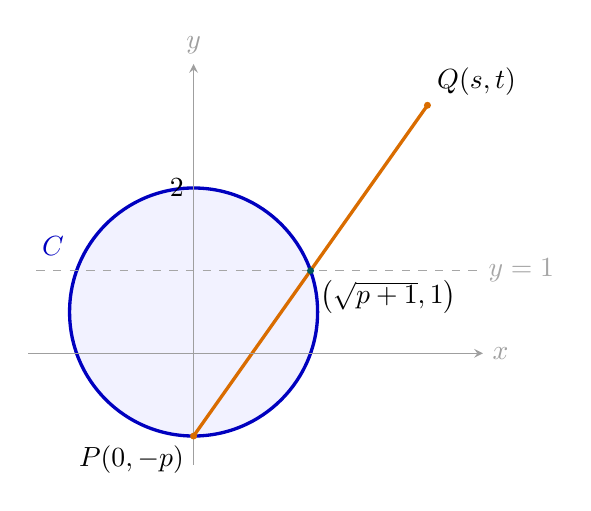
\begin{tikzpicture}[scale=1.05,>=stealth]
    % p=1 の代表図。C の中心は (0,1/2)，半径は 3/2。
    \coordinate (P) at (0,-1);
    \coordinate (B) at (1.4142,1);
    \coordinate (Q) at (2.8284,3);
    \fill[blue!5] (0,0.5) circle (1.5);
    \draw[blue!75!black,very thick] (0,0.5) circle (1.5);
    \draw[gray!70,dashed] (-1.9,1)--(3.45,1) node[right] {$y=1$};
    \draw[orange!85!black,very thick] (P)--(Q);
    \draw[->,gray!75] (-2,0)--(3.5,0) node[right] {$x$};
    \draw[->,gray!75] (0,-1.35)--(0,3.5) node[above] {$y$};
    \fill[orange!85!black] (P) circle (1.2pt) (Q) circle (1.2pt);
    \fill[teal!70!black] (B) circle (1.2pt);
    \node[below left] at (P) {$P(0,-p)$};
    \node[above right] at (Q) {$Q(s,t)$};
    \node[below right] at (B) {$\left(\sqrt{p+1},1\right)$};
    \node[blue!75!black,left] at (-1.45,1.3) {$C$};
    \node[left] at (0,2) {$2$};
  \end{tikzpicture}
  \caption{円 $C$ と直線 $PQ$ の位置関係（図は $p=1$）}
\end{figure}

\end{document}
